\documentclass[12pt]{scrartcl}
\usepackage{listings}
\usepackage{hyperref}
\usepackage{color}
\usepackage{graphicx}


\title{Python-exercises\\ C-Integration}

\newcommand{\ind}[1]{_{\mathrm{#1}}}

\begin{document}
\parindent0cm

\maketitle

\section{Compile an Example}

To check your setup, compile and run the examples 
\begin{itemize}
\item {\tt prime}
  \begin{itemize}
  \item use the manual way given in the talks, using {\tt primetest.c}
    and {\tt primewrap.c}
  \item use SWIG manually with {\tt primetest.i}
  \item automate this procedure with the {\tt setup.py} file
  \end{itemize}
\item {\tt vnorm}
  \begin{itemize}
  \item build manually with SWIG
  \item and use the {\tt setup.py} file
  \end{itemize}
\item {\tt dtw}.
\end{itemize}

Use the example modules to compare runtimes for the python
vs. c-implementation for one of the examples. Plot the runtimes of the
two implementations as a function of the input size.

\section{Python C-API}

\url{http://docs.python.org/c-api/index.html}

This exercise shows you that you can easily access python's
core-functionality from within C.

\subsection{List Example}
Translate the following python-code into C using the python c-api.

\lstinputlisting[language=python,caption=example1.py,frame=shadowbox]{solutions/c-api/example1.py}

\begin{enumerate}
\item use the high-level interface first ({\tt
  PyRun\_SimpleString()}\ldots)
\item use the object-interface.
\end{enumerate}

{\bf Note:} You need to call {\tt Py\_Initialize()} and {\tt
  Py\_Finalize()} at the beginning and at the end of your programs!

\subsection{Calculator}

Write a C-program using the Python C-API to write a calculator that
can evaluate a one-line expression (without variables) given as input
and prints the result.

Example call:

\begin{lstlisting}
mycalculator "2+sin(3*pi)/2-100"
Result of  2+sin(3*pi)/2-100 = -98.0
\end{lstlisting}

{\bf Note:} You need to put the argument in quotes!



\section{C-Module: Mean of random numbers}

Use SWIG for the following exercise:

\begin{enumerate}
\item Write a C-module {\tt float meanrand(long n)} that implements a function {\tt
  meanrand} that draws $n$ random real numbers (input to the function)
  from $[0,1]$ and returns their mean.
\item Write a second function {\tt float meanrand2( long n, float a, float b
  )} that draws $n$ random real numbers from $[a,b]$ and returns their
  mean.
\item Extend the interface to the second function with python-code
  such that you get the following default-arguments: {\tt
    meanrand.meanrand3( n=1000, a=0, b=1 )}
\item write a {\tt setup.py} file for this project
\item allow the user to set a seed for the random number generator
  with a function {\tt void setseed( unsigned int seed )}. Remember the
  seed in a global variable. In case {\tt seed=0}, use the current
  time as seed.
\item make a runtime-comparison with a pure python implementation as
  before, plotting $n$ vs. runtime

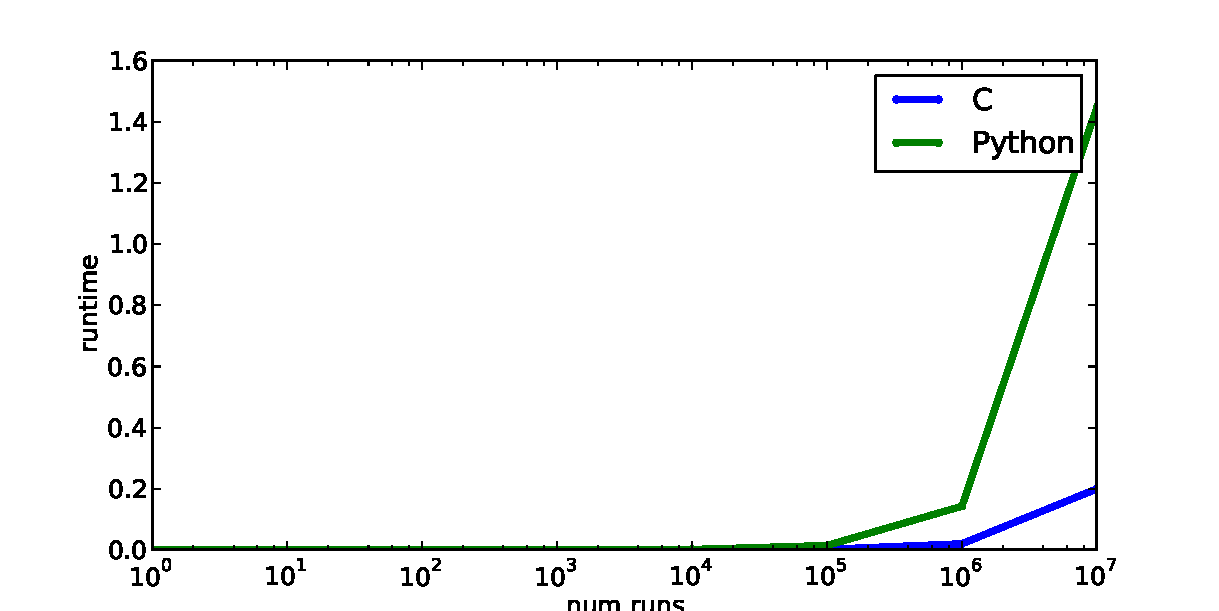
\includegraphics[width=.6\textwidth]{pics/meanrand}
\end{enumerate}


\section{C-Module: Geometric Mean}
Write a c-extension module {\tt geomean} that calculates the
  geometric mean
  \[
  G(x) = \sqrt[n]{x_1x_2\cdots x_n}.
  \]
\begin{enumerate}
\item Write function {\tt double geomean\_pow( double *x, int n )} and
  use a direct approach where you use the {\tt math.h} function {\tt
    pow} and the identity $\sqrt[n]{x}=x^{\frac{1}{n}}$.
\item Use the identity 
  \[
  \bigg(\prod_{i=1}^na_i \bigg)^{1/n} =
  \exp\left[\frac1n\sum_{i=1}^n\ln a_i\right]
  \]
  in function {\tt double geomean\_ln( double *x, int n)}.
\item Calculate $G$ for $n$ random numbers and plot the result as a
  function of $n$ for both functions. Add the result of {\tt
    scipy.stats.gmean} to the plot.
  
  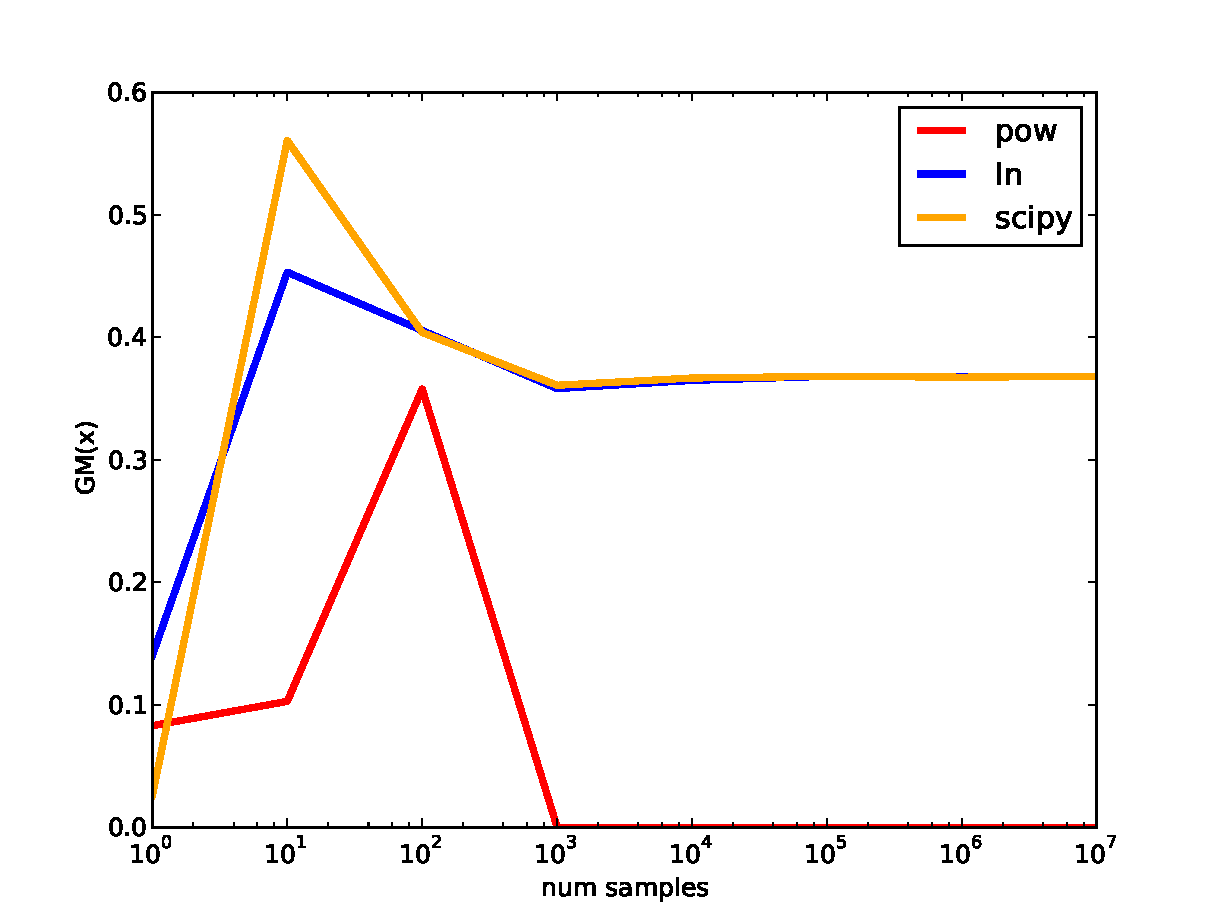
\includegraphics[width=.6\textwidth]{pics/geomean}
\end{enumerate}


{\bf Note:} Don't forget to copy {\tt numpy.i} into your folder!

\section{C-Module: Vector Addition}

Write a C-extension {\tt vecadd} that implements a function {\tt
  vecadd} that takes to numpy-vectors of length $n$ and returns the
element-wise sum of the vectors.

\begin{itemize}
\item Write a C-function with the signature {\tt int vecadd( float
  *v1, float *v2, int n, float *out )} where {\tt out} is a pointer to
  externally allocated memory and the return value is an error code (0
  if everything is ok). 
\item For accessing this function from python, you will need the numpy
  SWIG-typemaps, check out
  \url{http://docs.scipy.org/doc/numpy/reference/swig.interface-file.html}
  and the DTW example on the slides.
\item Write a c-function {\tt vecadd2} that calls {\tt vecadd} and has
  an interface that you can readily convert into numpy.i typemaps.
\item create the SWIG interface file for this function
\item Write appropriate python-code within the SWIG-interface file to
  provide a pythonic interface:
  
  {\tt v3=vecadd(v1,v2)}

  Do some checks in the python function that you need four your
  function to work properly (e.g., n1=n2, \ldots)
\end{itemize}

{\bf Note:} Don't forget to copy {\tt numpy.i} into your folder!

{\bf Note 2:} Be careful with the type of the numpy array! Ideally,
take care in the python-code from point (5) that the arrays are of the correct type!



\end{document}
